\chapter{Nutrición hídrica y mineral de las plantas}\label{ch:b1:plant-water-minerals}

Una planta de maíz en julio extrae un litro de agua al día de un suelo que
al tacto parece seco, y con ella los treinta miligramos de nitrógeno, en
forma de nitrato, que necesita para construir el crecimiento de un día. No
tiene \omterm{def:b1:membranes-transport:transporters}{bomba} alguna. El agua entra porque la \omterm{def:b1:flowering-plant-organization:organs}{raíz} está más seca que el suelo,
en el sentido preciso de \cref{ch:b1:membranes-transport}; el nitrato entra
porque las \omterm{def:b1:cell-unit-of-life:cell}{células} de la \omterm{def:b1:flowering-plant-organization:organs}{raíz} gastan \omterm{def:b1:water-small-molecules:atp}{ATP} para hacerlo entrar; y ambos deben
atravesar una sola capa de \omterm{def:b1:cell-unit-of-life:cell}{células} cuyas paredes están selladas con \omterm{def:b1:lipids:wax}{ceras}
antes de llegar al \omterm{def:b1:flowering-plant-organization:tissues}{xilema}. Este capítulo describe la \omterm{def:b1:flowering-plant-organization:organs}{raíz} como \omterm{def:b1:mammal-organization:organ}{órgano} de
\omterm{def:b1:digestion-absorption:nutrition}{absorción}, los \omterm{def:b1:membranes-transport:osmosis}{potenciales hídricos} que impulsan el agua del suelo al
\omterm{def:b1:flowering-plant-organization:tissues}{xilema}, los elementos minerales que una planta necesita y cómo los capta, el
caso particular del nitrógeno, y los hongos y bacterias que la mayoría de
las raíces emplean para hacer parte del trabajo.

\section{La raíz como órgano de absorción}

\begin{definition}[Apoplasto, simplasto, endodermis]\label{def:b1:plant-water-minerals:pathways}
\index{apoplasto}\index{simplasto}\index{banda de Caspary}
El agua y los solutos atraviesan el córtex de la \omterm{def:b1:flowering-plant-organization:organs}{raíz} por dos vías: el
\emph{apoplasto}, el sistema continuo de \omterm{prop:b1:carbohydrates:wall}{paredes celulares} y espacios
intercelulares, por el que se desplazan sin atravesar ninguna membrana; y el
\emph{simplasto}, el \omterm{def:b1:cell-unit-of-life:cell}{citoplasma} continuo de las \omterm{def:b1:cell-unit-of-life:cell}{células} conectadas por
\omterm{def:b1:eukaryotic-cell:plantcell}{plasmodesmos} (\cref{ch:b1:eukaryotic-cell}), en el que se entra atravesando
una membrana plasmática. En el límite interno del córtex, la
\emph{\omterm{prop:b1:flowering-plant-organization:stemroot}{endodermis}} (\cref{ch:b1:flowering-plant-organization}) bloquea el
apoplasto: una banda de suberina y lignina, la \emph{banda de Caspary},
impregna sus paredes radiales, de modo que todo lo que entra en el cilindro
vascular debe pasar por la membrana de una \omterm{def:b1:cell-unit-of-life:cell}{célula} endodérmica. Los
\omterm{def:b1:membranes-transport:transporters}{transportadores} de esa membrana deciden así lo que llega al \omterm{def:b1:flowering-plant-organization:tissues}{xilema}, e
impiden que lo cargado en el \omterm{def:b1:flowering-plant-organization:tissues}{xilema} se escape de vuelta.
\end{definition}

\begin{omfigure}
\begin{tikzpicture}[font=\footnotesize, >=Stealth, line cap=round]
  % row of cortex cells, endodermis, xylem
  \foreach \i in {0,1,2,3} {
    \draw[thick, omDef!60!black, fill=omDef!6] (1.6*\i,0) rectangle (1.6*\i+1.4,1.6);
    \draw[thick, omDef!60!black] (1.6*\i+0.15,0.15) rectangle (1.6*\i+1.25,1.45);
  }
  \node[anchor=south] at (2.9,1.7) {células del córtex (pared, luego membrana)};
  % endodermis cell with Casparian strip on radial walls
  \draw[thick, omDef!60!black, fill=omProp!12] (6.6,0) rectangle (8.0,1.6);
  \draw[thick, omDef!60!black] (6.75,0.15) rectangle (7.85,1.45);
  \draw[line width=4pt, omThm] (6.6,0.35) -- (6.6,1.25); \draw[line width=4pt, omThm] (8.0,0.35) -- (8.0,1.25);
  \node[anchor=south, align=center] at (7.3,1.7) {endodermis:\\ banda de Caspary (en rojo)};
  % xylem
  \draw[thick, omDef!60!black, fill=omDef!25] (8.4,0) rectangle (9.8,1.6);
  \node at (9.1,0.8) {xilema};
  % apoplast path: along walls, blocked at strip
  \draw[->, thick, omExo!70!black] (-0.6,0.08) -- (6.5,0.08);
  \draw[thick, omExo!70!black] (6.5,0.08) -- (6.5,0.3);
  \node[omExo!70!black, font=\scriptsize] at (6.2,-0.2) {bloqueado};
  \node[anchor=east, omExo!70!black, align=right, font=\scriptsize] at (-0.7,0.08) {apoplasto:\\ por las paredes};
  % symplast path: through cells via plasmodesmata
  \draw[->, thick, omProp!80!black] (-0.6,0.8) -- (0.15,0.8);
  \foreach \i in {0,1,2,3} { \draw[->, thick, omProp!80!black] (1.6*\i+1.25,0.8) -- (1.6*\i+1.75,0.8); }
  \draw[->, thick, omProp!80!black] (7.85,0.8) -- (8.4,0.8);
  \node[anchor=east, omProp!80!black, align=right, font=\scriptsize] at (-0.7,0.8) {simplasto:\\ por las células};
  % transfer from apoplast into symplast at endodermis
  \draw[->, thick, omThm] (6.4,0.25) -- (6.8,0.6);
  \node[anchor=north, align=center, gray] at (4.6,-0.5) {apoplasto: ninguna membrana hasta la endodermis, donde agua e iones deben entrar en una célula;\\ simplasto: una membrana en el pelo radical, luego plasmodesmos --- la célula elige lo que entra en el xilema};
\end{tikzpicture}

{\small Las dos vías a través del córtex de la \omterm{def:b1:flowering-plant-organization:organs}{raíz}. La vía apoplástica
discurre por las paredes hasta que la \omterm{def:b1:plant-water-minerals:pathways}{banda de Caspary} la detiene; la vía
simplástica atraviesa una membrana en la \omterm{def:b1:flowering-plant-organization:tissues}{epidermis} y luego va de \omterm{def:b1:cell-unit-of-life:cell}{célula} a
\omterm{def:b1:cell-unit-of-life:cell}{célula}. Ambas confluyen en las membranas de la \omterm{prop:b1:flowering-plant-organization:stemroot}{endodermis}.}
\end{omfigure}

\begin{proposition}[Presión radicular]\label{prop:b1:plant-water-minerals:rootpressure}
\index{presión radicular}\index{gutación}
La \omterm{prop:b1:flowering-plant-organization:stemroot}{endodermis} y las \omterm{def:b1:cell-unit-of-life:cell}{células} situadas por dentro de ella bombean iones hacia
el \omterm{def:b1:flowering-plant-organization:tissues}{xilema}, lo que rebaja el \omterm{def:b1:membranes-transport:osmosis}{potencial hídrico} del \omterm{def:b1:flowering-plant-organization:tissues}{xilema} y atrae agua por
\omterm{def:b1:membranes-transport:osmosis}{ósmosis} desde el córtex; cuando el vástago transpira poco (de noche, con el
aire húmedo), el agua se acumula y la savia del \omterm{def:b1:flowering-plant-organization:tissues}{xilema} es empujada hacia
arriba con una \emph{\omterm{prop:b1:plant-water-minerals:rootpressure}{presión radicular}} positiva de unas décimas de
megapascal --- suficiente para hacer salir gotas por los ápices de las \omterm{def:b1:flowering-plant-organization:organs}{hojas}
de las plantas pequeñas (la \emph{gutación}) y para rellenar vasos
bloqueados por aire, pero no para elevar la savia hasta la copa de un árbol.
De día toma el relevo la tracción de la transpiración
(\cref{ch:b1:plant-transport}) y la \omterm{prop:b1:plant-water-minerals:rootpressure}{presión radicular} desaparece.
\end{proposition}
\begin{proof}[Evidencia]
Un \omterm{def:b1:flowering-plant-organization:organs}{tallo} cortado cerca del suelo exuda savia durante horas desde su tocón, y
un manómetro acoplado al tocón registra una presión de
\qtyrange{0.1}{0.3}{MPa}; el exudado es más rico en iones que la disolución
del suelo, y su flujo cesa cuando las raíces se enfrían o se envenenan con
un \omterm{def:b1:enzymes:inhibitors}{inhibidor} de la respiración: el flujo lo impulsa la carga activa de
iones, y no bombeo alguno de agua.
\end{proof}

\section{El agua: del suelo al xilema}

\begin{proposition}[La escalera de potencial hídrico]\label{prop:b1:plant-water-minerals:ladder}
\index{potencial hídrico}
El agua va del suelo al \omterm{def:b1:flowering-plant-organization:tissues}{xilema} porque el \omterm{def:b1:membranes-transport:osmosis}{potencial hídrico}
(\cref{ch:b1:membranes-transport}) desciende en cada peldaño:
\begin{center}
\small
\begin{tabular}{lr}
\hline
compartimento & $\Psi$ (\unit{MPa}) \\
\hline
suelo húmedo & $-0.03$ a $-0.3$ \\
suelo en el punto de marchitez & $-1.5$ \\
\omterm{def:b1:cell-unit-of-life:cell}{célula} del córtex radical & $-0.3$ a $-0.6$ \\
\omterm{def:b1:flowering-plant-organization:tissues}{xilema} de la \omterm{def:b1:flowering-plant-organization:organs}{raíz} & $-0.5$ a $-0.8$ \\
\omterm{def:b1:cell-unit-of-life:cell}{células} de la \omterm{def:b1:flowering-plant-organization:organs}{hoja} & $-1.0$ a $-2.0$ \\
aire al \qty{50}{\%} de humedad relativa & $-95$ \\
\hline
\end{tabular}
\end{center}
El potencial del suelo lo fija sobre todo la tensión con que sus poros
retienen el agua (la capilaridad); el de las \omterm{def:b1:cell-unit-of-life:cell}{células}, sus solutos y su
\omterm{def:b1:eukaryotic-cell:plantcell}{turgencia}; el del \omterm{def:b1:flowering-plant-organization:tissues}{xilema}, la tensión de la columna que transpira; el del
aire, su humedad, $\Psi = (RT/V_w)\ln(\text{HR})$, que es enorme incluso con
aire húmedo. El peldaño más pronunciado con diferencia es el último, de la
\omterm{def:b1:flowering-plant-organization:organs}{hoja} al aire: ahí se gasta casi toda la fuerza impulsora, y por eso las
plantas lo controlan con los \omterm{def:b1:flowering-plant-organization:tissues}{estomas}.
\end{proposition}

\begin{omfigure}
\begin{tikzpicture}
\begin{axis}[
  ybar, bar width=14pt,
  width=0.86\linewidth, height=5.8cm,
  axis x line=bottom, axis y line=left,
  ymin=-2.2, ymax=0.2,
  ylabel={potencial hídrico $\Psi$ (\unit{MPa})},
  ylabel style={font=\small},
  symbolic x coords={suelo, córtex radical, xilema radical, xilema del tallo, célula foliar, aire de la hoja},
  xtick=data, x tick label style={font=\small, rotate=20, anchor=north east},
  enlarge x limits=0.12, ytick={0,-0.5,-1,-1.5,-2},
  nodes near coords, nodes near coords style={font=\scriptsize, anchor=north},
  point meta=rawy,
  clip=false,
]
\addplot[fill=omDef!45, draw=omDef] coordinates {(suelo,-0.2) (córtex radical,-0.4) (xilema radical,-0.6) (xilema del tallo,-0.9) (célula foliar,-1.3) (aire de la hoja,-1.5)};
\node[font=\scriptsize, anchor=west, align=left, xshift=9pt] at (axis cs:aire de la hoja,-0.3) {(aire exterior:\\ $-95$, fuera de escala)};
\end{axis}
\end{tikzpicture}

{\small \omterm{def:b1:membranes-transport:osmosis}{Potencial hídrico} a lo largo del recorrido por una planta de maíz
que transpira en un día de verano. Cada peldaño es más bajo que el anterior;
la caída hacia el aire exterior, cien veces mayor que todas las demás
juntas, no está dibujada.}
\end{omfigure}

\begin{method}[Lectura de un perfil de potencial hídrico]\label{met:b1:plant-water-minerals:profile}
\begin{enumerate}
  \item Enumérense los compartimentos en orden con su $\Psi$; el agua fluye
        solo de mayor a menor, de modo que la secuencia debe decrecer a lo
        largo del recorrido, o el flujo se invierte.
  \item Sepárese el $\Psi$ de cada \omterm{def:b1:cell-unit-of-life:cell}{célula} en $\Psi_s$ (solutos, negativo) y
        $\Psi_p$ (\omterm{def:b1:eukaryotic-cell:plantcell}{turgencia}, positivo); una \omterm{def:b1:cell-unit-of-life:cell}{célula} de la \omterm{def:b1:flowering-plant-organization:organs}{raíz} a $\Psi = -0.4$ con $\Psi_s = -0.9$ tiene $\Psi_p = +0.5$. El agua del \omterm{def:b1:flowering-plant-organization:tissues}{xilema}
        tiene $\Psi_s \approx 0$ y un $\Psi_p$ negativo: está bajo tensión.
  \item El flujo a través de un peldaño es la diferencia de $\Psi$ por la
        conductancia hidráulica de la barrera; la \omterm{prop:b1:flowering-plant-organization:stemroot}{endodermis} y los \omterm{def:b1:flowering-plant-organization:tissues}{estomas}
        son los dos peldaños de baja conductancia donde la planta regula.
  \item Séquese el suelo y su $\Psi$ desciende; cuando alcanza el de la
        \omterm{def:b1:flowering-plant-organization:organs}{hoja}, el flujo se detiene y la planta se marchita; cuando el
        $\Psi_p$ de las \omterm{def:b1:cell-unit-of-life:cell}{células} de la \omterm{def:b1:flowering-plant-organization:organs}{hoja} llega a cero, la \omterm{def:b1:flowering-plant-organization:organs}{hoja} cuelga. La
        recuperación exige que cambie el suelo, no la planta.
\end{enumerate}
\end{method}

\begin{example}[Un litro al día]\label{ex:b1:plant-water-minerals:litre}
Las raíces finas de una planta de maíz ofrecen unos \qty{0.2}{m^2} de
superficie con una conductancia hidráulica de unos
\qty{2e-7}{m.s^{-1}.MPa^{-1}}; entre un suelo a \qty{-0.2}{MPa} y un \omterm{def:b1:flowering-plant-organization:tissues}{xilema}
radical a \qty{-0.6}{MPa} el flujo es $2\times 10^{-7}\times 0.4\times 0.2 = \qty{1.6e-8}{m^3/s}$ --- litro y medio al día, todo él perdido por las
\omterm{def:b1:flowering-plant-organization:organs}{hojas}. La \omterm{def:b1:flowering-plant-organization:organs}{raíz} no realiza trabajo alguno para moverlo: la transpiración de
la \omterm{def:b1:flowering-plant-organization:organs}{hoja} fija la tensión, y el suelo aporta el agua mientras su potencial se
mantenga por encima del de la \omterm{def:b1:flowering-plant-organization:organs}{raíz}.
\end{example}

\section{Nutrición mineral}

\begin{definition}[Elementos esenciales]\label{def:b1:plant-water-minerals:elements}
\index{elemento esencial}\index{macronutriente}\index{micronutriente}
Un elemento es \emph{esencial} para una planta si esta no puede completar su
ciclo vital sin él y ningún otro elemento puede sustituirlo. Son diecisiete:
carbono, hidrógeno y oxígeno, del aire y del agua; los
\emph{macronutrientes}, tomados del suelo en gramos por kilogramo de masa
seca --- nitrógeno (como nitrato o amonio), fósforo (fosfato), potasio,
calcio, magnesio, azufre (sulfato); y los \emph{micronutrientes}, necesarios
en miligramos o menos --- hierro, manganeso, cinc, cobre, boro, molibdeno,
cloro, níquel. El nitrógeno construye \omterm{def:b1:proteins:peptide}{proteínas} y ácidos nucleicos; el
fósforo, \omterm{def:b1:nucleic-acids:nucleotide}{nucleótidos} y membranas; el potasio es el principal catión de la
\omterm{def:b1:cell-unit-of-life:cell}{célula} y el agente osmótico de los \omterm{def:b1:flowering-plant-organization:tissues}{estomas}; el magnesio ocupa el centro de
la \omterm{def:b1:photosynthesis:pigments}{clorofila}; el hierro, los citocromos y la ferredoxina; el molibdeno, la
\omterm{prop:b1:plant-water-minerals:nitrate}{nitrato-reductasa} y la nitrogenasa.
\end{definition}

\begin{proposition}[Cómo se elaboró la lista]\label{prop:b1:plant-water-minerals:hydroponics}
Los \omterm{def:b1:plant-water-minerals:elements}{elementos esenciales} se identificaron cultivando plantas en agua que
contenía únicamente sales conocidas.
\end{proposition}
\begin{proof}[Evidencia]
Sachs y Knop (década de 1860) cultivaron plantas hasta la madurez en
disoluciones de unas pocas sales minerales, sin suelo alguno, y demostraron
así que el suelo no aporta más que minerales y sostén; suprimir una sal cada
vez daba una dolencia característica para cada elemento, y devolverla la
curaba. Los \omterm{def:b1:plant-water-minerals:elements}{micronutrientes} se descubrieron más tarde, a medida que los
químicos aprendieron a purificar las sales: una planta privada de molibdeno,
necesario en una parte por diez millones, no consigue reducir el nitrato. La
técnica, la hidroponía, alimenta hoy invernaderos.
\end{proof}

\begin{omfigure}
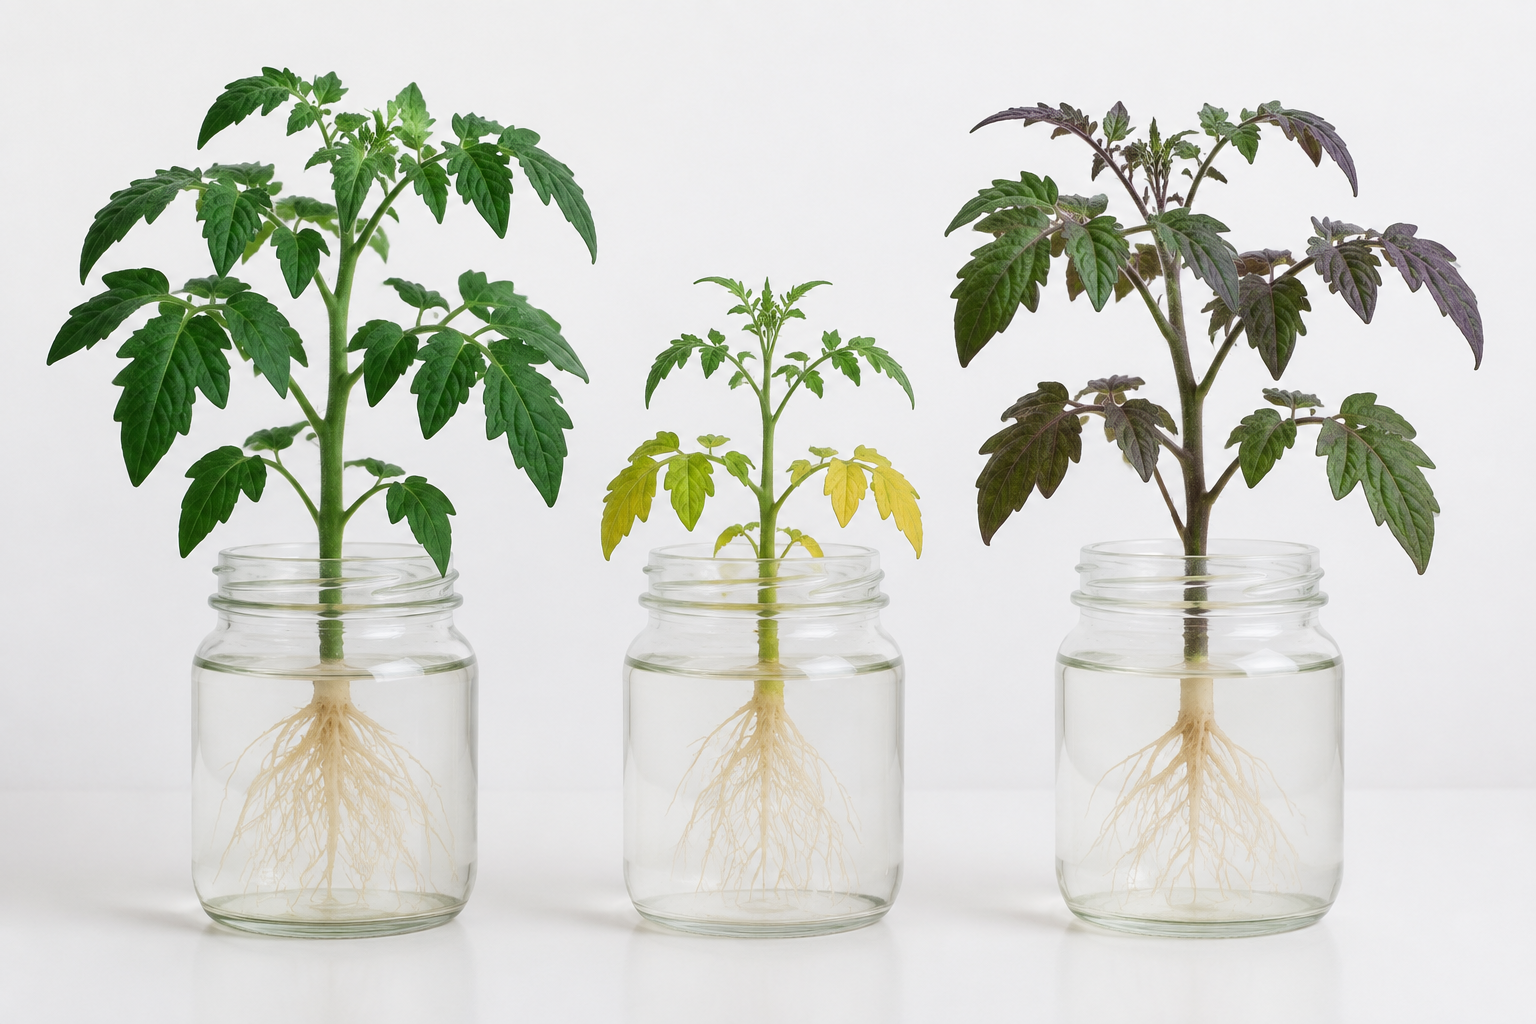
\includegraphics[width=0.6\linewidth]{images/book3/ai/b3-23-nutrient-deficiency.png}

{\small Tres tomateras en disoluciones nutritivas: completa (izquierda), sin
nitrógeno (centro: raquítica, con las \omterm{def:b1:flowering-plant-organization:organs}{hojas} viejas amarillas porque su
nitrógeno se traslada a las jóvenes), sin fósforo (derecha: \omterm{def:b1:flowering-plant-organization:organs}{hojas} oscuras
con tintes purpúreos). Cada elemento que falta tiene su firma.}
\end{omfigure}

\begin{method}[Lectura de una carencia]\label{met:b1:plant-water-minerals:deficiency}
\begin{enumerate}
  \item Pregúntese dónde aparece el síntoma. Los elementos que la planta
        puede movilizar por el floema (N, P, K, Mg) se retiran de las \omterm{def:b1:flowering-plant-organization:organs}{hojas}
        viejas para alimentar a las jóvenes: las \omterm{def:b1:flowering-plant-organization:organs}{hojas} viejas muestran
        primero la carencia. Los que no puede movilizar (Ca, Fe, B) quedan
        varados donde se depositaron: la muestran las \omterm{def:b1:flowering-plant-organization:organs}{hojas} jóvenes y los
        ápices en crecimiento.
  \item Pregúntese qué hace el elemento: sin nitrógeno, poca \omterm{def:b1:photosynthesis:pigments}{clorofila} y
        poca \omterm{def:b1:proteins:peptide}{proteína} --- planta pálida y raquítica; sin magnesio o hierro,
        falla la \omterm{def:b1:photosynthesis:pigments}{clorofila} --- \omterm{def:b1:flowering-plant-organization:organs}{hojas} amarillas con los nervios verdes; sin
        potasio, los bordes de la \omterm{def:b1:flowering-plant-organization:organs}{hoja} se queman; sin calcio, mueren los
        ápices en crecimiento.
  \item Confírmese aportando solo el elemento sospechoso y observando el
        crecimiento nuevo.
\end{enumerate}
\end{method}

\begin{proposition}[Captación activa de iones]\label{prop:b1:plant-water-minerals:uptake}
\index{bomba de protones}
La disolución del suelo contiene los iones a micromoles o unos pocos
milimoles por litro; las \omterm{def:b1:cell-unit-of-life:cell}{células} de la \omterm{def:b1:flowering-plant-organization:organs}{raíz} retienen el potasio a
\qty{100}{mmol/L}, el fosfato a \qty{10}{} y el nitrato a varios. La
captación es por tanto casi siempre cuesta arriba y se paga con \omterm{def:b1:water-small-molecules:atp}{ATP}, pero de
manera indirecta: una \emph{\omterm{prop:b1:plant-water-minerals:uptake}{bomba de protones}} de la membrana plasmática
(\cref{ch:b1:membranes-transport}) exporta $\mathrm{H^+}$, lo que acidifica
el exterior y deja el interior negativo en
\qtyrange{-120}{-200}{mV}; los cationes como el $\mathrm{K^+}$ entran
entonces por \omterm{def:b1:membranes-transport:transporters}{canales} a favor del gradiente eléctrico, y los aniones
($\mathrm{NO_3^-}$, $\mathrm{H_2PO_4^-}$, $\mathrm{SO_4^{2-}}$) por
\omterm{prop:b1:membranes-transport:secondary}{simportadores} que aprovechan la vuelta de los protones. Los \omterm{def:b1:membranes-transport:transporters}{transportadores}
son selectivos: el potasio se capta cien veces mejor que el sodio, de igual
carga y tamaño casi idéntico, y la planta mantiene fuera el sodio incluso en
suelo salino. Las raíces dedican a este transporte un tercio de la
respiración de la planta.
\end{proposition}

\section{El nitrógeno}

\begin{proposition}[Del nitrato al aminoácido]\label{prop:b1:plant-water-minerals:nitrate}
\index{nitrato-reductasa}\index{asimilación del nitrógeno}
La mayoría de las plantas toman el nitrógeno como nitrato. En el \omterm{def:b1:eukaryotic-cell:organelle}{citosol}, la
\emph{\omterm{prop:b1:plant-water-minerals:nitrate}{nitrato-reductasa}}, una \omterm{def:b1:enzymes:enzyme}{enzima} con molibdeno, lo reduce a nitrito con
electrones del NADH; en el \omterm{def:b1:eukaryotic-cell:plastid}{plasto}, la \emph{nitrito-reductasa} reduce el
nitrito a amonio con electrones de la ferredoxina; y el amonio se fija de
inmediato en glutamina y \omterm{def:b1:biosyntheses-integration:nitrogen}{glutamato}
(\cref{ch:b1:biosyntheses-integration}) --- el amonio en sí es tóxico y
nunca se acumula. La reducción completa cuesta ocho electrones por
nitrógeno, una décima parte del flujo fotosintético de electrones de una
\omterm{def:b1:flowering-plant-organization:organs}{hoja} en un suelo rico en nitrato, y la \omterm{def:b1:flowering-plant-organization:organs}{hoja} realiza buena parte de ella a la
luz, directamente desde la ferredoxina del cloroplasto. El amonio, donde el
suelo lo ofrece, se capta directamente y ahorra ese coste.
\end{proposition}

\begin{definition}[Fijación del nitrógeno y nódulos]\label{def:b1:plant-water-minerals:nodules}
\index{fijación del nitrógeno}\index{nódulo radicular}\index{Rhizobium}
Ningún eucariota puede usar el $\mathrm{N_2}$ del aire. Algunas bacterias
sí: la \emph{nitrogenasa} rompe el triple enlace del $\mathrm{N_2}$ y lo
reduce a dos amoníacos, a un coste de dieciséis \omterm{def:b1:water-small-molecules:atp}{ATP} y ocho electrones por
molécula, y solo donde el oxígeno queda excluido. Las leguminosas
(guisantes, judías, trébol) alojan esas bacterias (\emph{Rhizobium}) en
\emph{nódulos radiculares}: la planta construye una cámara, alimenta con
azúcar a las bacterias y mantiene bajo el oxígeno con una \omterm{def:b1:proteins:peptide}{proteína} roja, la
leghemoglobina, que se lo entrega a la respiración bacteriana a una
concentración demasiado baja para dañar la \omterm{def:b1:enzymes:enzyme}{enzima}; las bacterias devuelven
amonio, que la planta convierte en \omterm{def:b1:proteins:aminoacid}{aminoácidos}. Un campo de trébol fija cien
kilogramos de nitrógeno por hectárea y año, por los que la planta paga una
décima parte de su fotosíntesis. El ciclo del nitrógeno en su conjunto
pertenece al volumen de segundo año.
\end{definition}

\begin{omfigure}
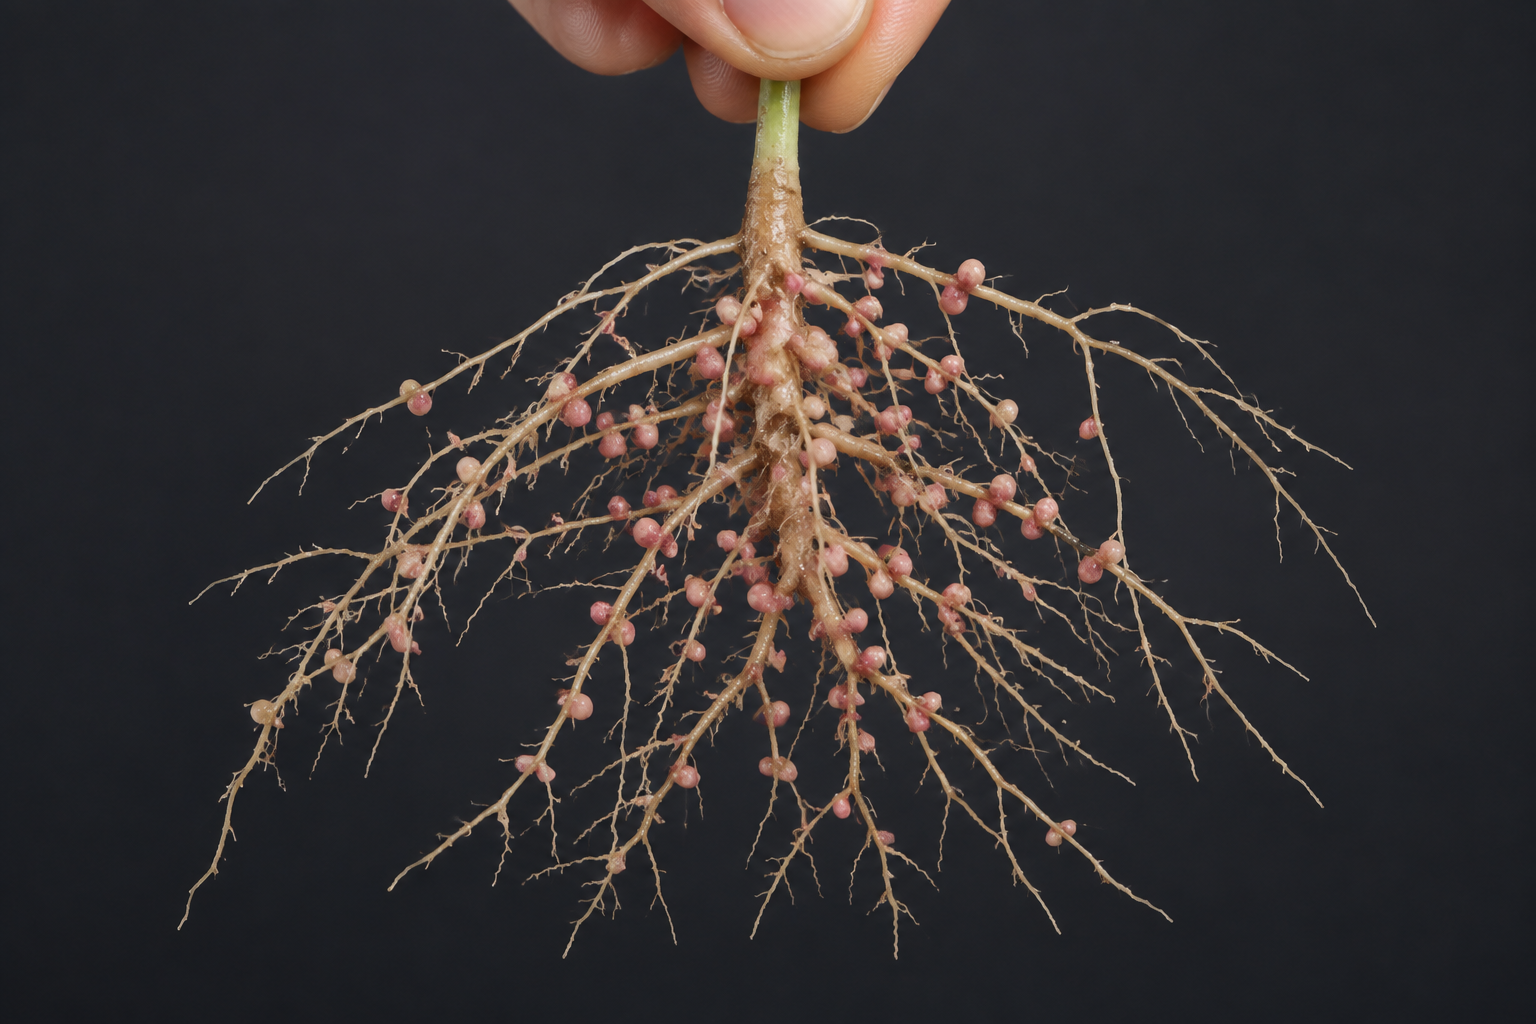
\includegraphics[width=0.52\linewidth]{images/book3/ai/b3-23-root-nodules.png}

{\small Nódulos en las raíces de una leguminosa: cada uno es una cámara de
\omterm{def:b1:body-plans-tissues:tissue}{tejido} vegetal llena de bacterias, rosada por la leghemoglobina, donde se
fija el nitrógeno atmosférico.}
\end{omfigure}

\begin{example}[El precio del nitrógeno]\label{ex:b1:plant-water-minerals:priceN}
Una planta de maíz necesita unos \qty{30}{mg} de nitrógeno al día; de un
nitrato a \qty{2}{mmol/L} los obtiene en el litro de agua que transpira, y
gasta unos cientos de milimoles de electrones en reducirlo. Un trébol que
fije la misma cantidad paga \qty{16}{} \omterm{def:b1:water-small-molecules:atp}{ATP} por $\mathrm{N_2}$ más el
reductor --- unos \qty{6}{g} de azúcar por gramo de nitrógeno, unos
\qty{0.2}{g} al día, una décima parte de su producción --- y puede crecer en
un suelo sin nada de nitrato. Los agricultores llevan dos mil años alternando
leguminosas con cereales para llevar ese nitrógeno de un campo al siguiente.
\end{example}

\section{Socios en el suelo}

\begin{definition}[Micorriza]\label{def:b1:plant-water-minerals:mycorrhiza}
\index{micorriza}
Una \emph{micorriza} es una asociación entre una \omterm{def:b1:flowering-plant-organization:organs}{raíz} y un hongo, presente
en nueve plantas de cada diez. En la forma más común, las hifas del hongo
crecen hacia el interior de las \omterm{def:b1:cell-unit-of-life:cell}{células} del córtex y se ramifican dentro de
ellas en \emph{arbúsculos}, la \omterm{prop:b1:organism-environment:surfaces}{superficie de intercambio}, mientras que fuera
de la \omterm{def:b1:flowering-plant-organization:organs}{raíz} una red de hifas de unos pocos micrómetros de grosor explora el
suelo a lo largo de metros. El hongo entrega fosfato y otros iones poco
móviles, y agua, adonde los propios pelos de la \omterm{def:b1:flowering-plant-organization:organs}{raíz} no llegarían; la planta
entrega azúcar, una décima parte o más de su fotosíntesis. Los árboles de
los bosques templados llevan una segunda forma, en la que el hongo envuelve
los ápices radicales y se intercala entre las \omterm{def:b1:cell-unit-of-life:cell}{células}; sus cuerpos
fructíferos son las setas del suelo del bosque.
\end{definition}
\begin{proof}[Evidencia]
Las plántulas cultivadas en suelo esterilizado crecen mal y captan poco
fosfato; inoculadas con esporas del hongo, crecen varias veces más. Un
fosfato radiactivo colocado en el suelo fuera del alcance de las raíces
aparece en la planta solo si hay hifas que conecten ambos puntos, y un
carbono marcado suministrado a las \omterm{def:b1:flowering-plant-organization:organs}{hojas} aparece en las hifas en un día.
Cortar las hifas con una malla fina que deja pasar los solutos pero no los
hongos suprime la ganancia.
\end{proof}

\begin{omfigure}
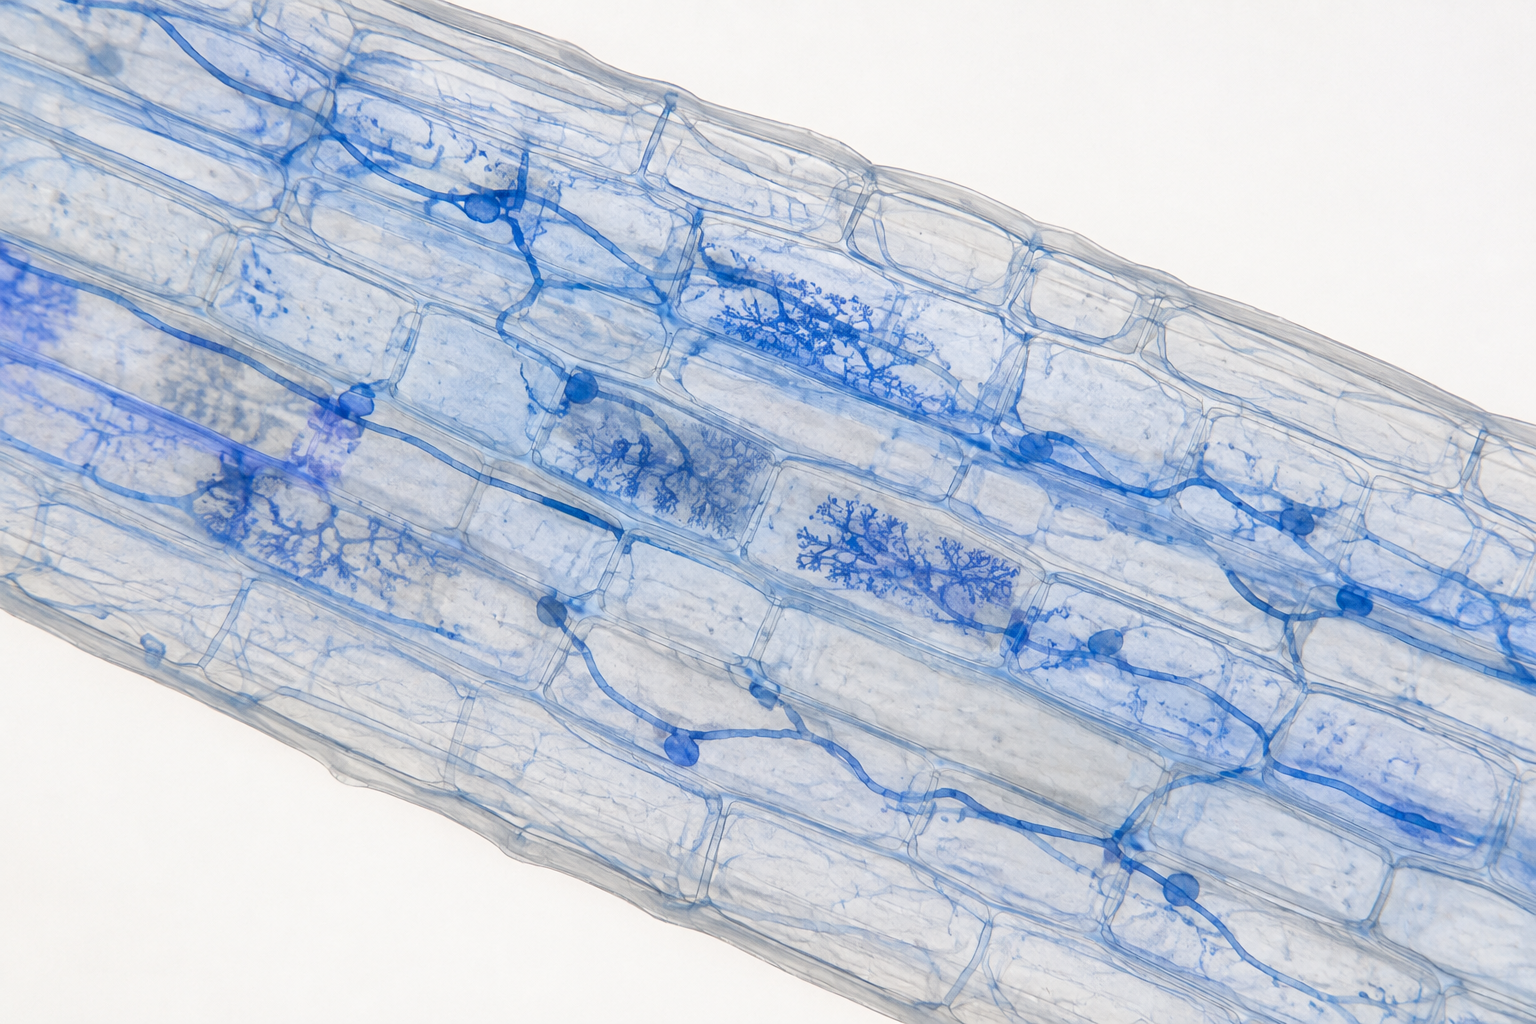
\includegraphics[width=0.52\linewidth]{images/book3/ai/b3-23-mycorrhiza.png}

{\small Una \omterm{def:b1:flowering-plant-organization:organs}{raíz} teñida para mostrar su hongo micorrícico: hifas que corren
entre las \omterm{def:b1:cell-unit-of-life:cell}{células} y se ramifican en arbúsculos dentro de ellas --- una
segunda superficie de \omterm{def:b1:digestion-absorption:nutrition}{absorción}, abastecida de azúcar por la planta.}
\end{omfigure}

\begin{example}[Por qué el fosfato necesita un hongo]\label{ex:b1:plant-water-minerals:phosphate}
El fosfato se une a las partículas del suelo y difunde un milímetro al día;
un \omterm{def:b1:flowering-plant-organization:organs}{pelo radical} capta en unas horas todo el fosfato a su alcance y luego
espera. Unas hifas diez veces más finas que un \omterm{def:b1:flowering-plant-organization:organs}{pelo radical} llegan diez
veces más lejos por gramo de \omterm{def:b1:body-plans-tissues:tissue}{tejido}, y un metro de hifa le cuesta a la
planta la milésima parte de lo que le cuesta un metro de \omterm{def:b1:flowering-plant-organization:organs}{raíz}. Para el
nitrato, que se mueve libremente con el agua del suelo, bastan los propios
pelos de la \omterm{def:b1:flowering-plant-organization:organs}{raíz}, y las plantas de suelos ricos en nitrato reducen su hongo;
para el fosfato, el hongo es la prolongación de la \omterm{def:b1:flowering-plant-organization:organs}{raíz}.
\end{example}

\section{Ejercicios}

\begin{exercise}[$\star$]\label{exo:b1:plant-water-minerals:1}
Defínanse \omterm{def:b1:plant-water-minerals:pathways}{apoplasto} y \omterm{def:b1:plant-water-minerals:pathways}{simplasto}, y dígase qué hace la \omterm{def:b1:plant-water-minerals:pathways}{banda de Caspary}.
\end{exercise}

\begin{exercise}[$\star$]\label{exo:b1:plant-water-minerals:2}
Enumérense los seis \omterm{def:b1:plant-water-minerals:elements}{macronutrientes} que una planta toma del suelo y una
función de cada uno.
\end{exercise}

\begin{exercise}[$\star$]\label{exo:b1:plant-water-minerals:3}
A partir de la figura del \omterm{def:b1:membranes-transport:osmosis}{potencial hídrico}, léase $\Psi$ en el suelo, en el
\omterm{def:b1:flowering-plant-organization:tissues}{xilema} de la \omterm{def:b1:flowering-plant-organization:organs}{raíz} y en la \omterm{def:b1:cell-unit-of-life:cell}{célula} de la \omterm{def:b1:flowering-plant-organization:organs}{hoja}, y enúnciese el sentido del
flujo en cada peldaño.
\end{exercise}

\begin{exercise}[$\star$]\label{exo:b1:plant-water-minerals:4}
¿Por qué la carencia de nitrógeno y la de hierro se manifiestan en \omterm{def:b1:flowering-plant-organization:organs}{hojas}
distintas?
\end{exercise}

\begin{exercise}[$\star\star$]\label{exo:b1:plant-water-minerals:5}
Una \omterm{def:b1:cell-unit-of-life:cell}{célula} del córtex radical tiene $\Psi_s = \qty{-0.9}{MPa}$ y $\Psi_p =
\qty{0.5}{MPa}$; el suelo está a \qty{-0.2}{MPa} y el \omterm{def:b1:flowering-plant-organization:tissues}{xilema} a
\qty{-0.6}{MPa}. Demuéstrese que el agua fluye del suelo a la \omterm{def:b1:cell-unit-of-life:cell}{célula} y de
esta al \omterm{def:b1:flowering-plant-organization:tissues}{xilema}, y calcúlese el $\Psi_p$ de la \omterm{def:b1:cell-unit-of-life:cell}{célula} al que dejaría de
captar agua de este suelo.
\end{exercise}

\begin{exercise}[$\star\star$]\label{exo:b1:plant-water-minerals:6}
Calcúlese el \omterm{def:b1:membranes-transport:osmosis}{potencial hídrico} del aire al \qty{90}{\%}, al \qty{50}{\%} y
al \qty{10}{\%} de humedad relativa a \qty{25}{\celsius} ($RT/V_w =
\qty{137}{MPa}$). Compárese con el suelo en el punto de marchitez y
coméntese.
\end{exercise}

\begin{exercise}[$\star\star$]\label{exo:b1:plant-water-minerals:7}
Una \omterm{def:b1:cell-unit-of-life:cell}{célula} de la \omterm{def:b1:flowering-plant-organization:organs}{raíz} a \qty{-150}{mV} capta $\mathrm{K^+}$ desde
\qty{0.1}{mmol/L} hasta \qty{100}{mmol/L}. Calcúlese el potencial de Nernst
para esa relación a \qty{25}{\celsius} y dígase si bastan los \omterm{def:b1:membranes-transport:transporters}{canales} por sí
solos. Repítase para el nitrato, a \qty{0.5}{} fuera y \qty{5}{mmol/L}
dentro.
\end{exercise}

\begin{exercise}[$\star\star$]\label{exo:b1:plant-water-minerals:8}
Explíquese por qué se ve gutación al amanecer en la hierba pero nunca en un
árbol alto, y qué le ocurre a la \omterm{prop:b1:plant-water-minerals:rootpressure}{presión radicular} cuando empieza la
transpiración.
\end{exercise}

\begin{exercise}[$\star\star$]\label{exo:b1:plant-water-minerals:9}
Se traslada una planta a una disolución sin molibdeno. Predígase su
crecimiento sobre nitrato y sobre amonio, y explíquese la diferencia.
\end{exercise}

\begin{exercise}[$\star\star\star$]\label{exo:b1:plant-water-minerals:10}
Calcúlense los electrones necesarios para reducir a amonio \qty{30}{mg} de
nitrógeno nítrico al día, y los equivalentes de \omterm{def:b1:biosyntheses-integration:ppp}{NADPH}; compárense con los
electrones que una \omterm{def:b1:flowering-plant-organization:organs}{hoja} de maíz de \qty{500}{cm^2} hace pasar por sus
\omterm{def:b1:photosynthesis:zscheme}{fotosistemas} en un día a \qty{4}{\micro mol} de $\mathrm{CO_2}$ por metro
cuadrado y segundo (4 electrones por $\mathrm{CO_2}$, \qty{12}{h}).
\end{exercise}

\begin{exercise}[$\star\star\star$]\label{exo:b1:plant-water-minerals:11}
Un trébol fija \qty{30}{mg} de nitrógeno al día a \qty{16}{} \omterm{def:b1:water-small-molecules:atp}{ATP} y
\qty{8}{} electrones por $\mathrm{N_2}$, y \qty{6}{g} de azúcar por gramo de
nitrógeno en total. Calcúlense el \omterm{def:b1:water-small-molecules:atp}{ATP} que gasta la nitrogenasa por sí sola,
el azúcar que costaría (30 \omterm{def:b1:water-small-molecules:atp}{ATP} por glucosa) y la fracción de los \qty{6}{g}
que eso representa. ¿Adónde va el resto?
\end{exercise}

\begin{exercise}[$\star\star\star$]\label{exo:b1:plant-water-minerals:12}
``Una \omterm{def:b1:flowering-plant-organization:organs}{raíz} es una explotación minera que subcontrata.'' Discútase en un
párrafo: qué hace la \omterm{def:b1:flowering-plant-organization:organs}{raíz} por sí misma (agua, iones móviles), qué
subcontrata (fosfato, nitrógeno fijado), qué paga y cuándo deja de pagar.
\end{exercise}

\section{Problema: la escalera de potencial hídrico de una raíz de maíz}

\begin{problem}[{Problema de fin de semana --- agua y nitrato de un suelo de
julio hacia una planta de maíz: potenciales en cada peldaño, el flujo a
través de las raíces, el nitrógeno que transporta y el coste de reducirlo,
hasta llegar al flujo diario de agua hacia la raíz}]
\label{pb:b1:plant-water-minerals:1}
Una planta de maíz en julio: superficie de raíces finas \qty{0.2}{m^2},
conductancia hidráulica de la \omterm{def:b1:flowering-plant-organization:organs}{raíz} \qty{2e-7}{m.s^{-1}.MPa^{-1}}; superficie
foliar \qty{0.5}{m^2}. \omterm{def:b1:membranes-transport:osmosis}{Potencial hídrico} del suelo \qty{-0.2}{MPa}; \omterm{def:b1:cell-unit-of-life:cell}{células}
del córtex radical con $\Psi_s = \qty{-0.9}{MPa}$ y $\Psi_p = \qty{0.5}{MPa}$; \omterm{def:b1:flowering-plant-organization:tissues}{xilema} de la \omterm{def:b1:flowering-plant-organization:organs}{raíz} \qty{-0.6}{MPa}; \omterm{def:b1:cell-unit-of-life:cell}{células} de la \omterm{def:b1:flowering-plant-organization:organs}{hoja}
\qty{-1.3}{MPa}; aire al \qty{50}{\%} de humedad relativa ($RT/V_w = \qty{137}{MPa}$). Nitrato del suelo \qty{2}{mmol/L}; la planta necesita
\qty{30}{mg} de nitrógeno al día. La reducción del nitrato a amonio consume
8 electrones por nitrógeno; la fotosíntesis mueve 4 electrones por
$\mathrm{CO_2}$ y la \omterm{def:b1:flowering-plant-organization:organs}{hoja} fija \qty{4}{\micro mol} de $\mathrm{CO_2}$ por
metro cuadrado y segundo durante \qty{12}{h}.

\medskip
\noindent\textbf{Parte I --- La escalera.}
\begin{enumerate}
  \item Calcúlese el \omterm{def:b1:membranes-transport:osmosis}{potencial hídrico} de las \omterm{def:b1:cell-unit-of-life:cell}{células} del córtex radical.
  \item Escríbase la secuencia suelo, córtex, \omterm{def:b1:flowering-plant-organization:tissues}{xilema}, \omterm{def:b1:flowering-plant-organization:organs}{hoja}, y compruébese
        que el agua fluye hacia dentro y hacia arriba en cada peldaño.
  \item Calcúlese el \omterm{def:b1:membranes-transport:osmosis}{potencial hídrico} del aire.
  \item Calcúlense la caída del suelo a la \omterm{def:b1:flowering-plant-organization:organs}{hoja} y la caída de la \omterm{def:b1:flowering-plant-organization:organs}{hoja} al
        aire; ¿qué fracción del total es el último peldaño?
  \item El suelo se seca hasta \qty{-0.9}{MPa}. ¿Qué ocurre con el flujo
        hacia las \omterm{def:b1:cell-unit-of-life:cell}{células} del córtex, y con su \omterm{def:b1:eukaryotic-cell:plantcell}{turgencia}?
  \item El suelo se seca hasta \qty{-1.5}{MPa}. ¿Qué les ocurre a las \omterm{def:b1:flowering-plant-organization:organs}{hojas},
        y por qué las restaura el riego?
\end{enumerate}

\medskip
\noindent\textbf{Parte II --- El flujo.}
\begin{enumerate}[resume]
  \item Calcúlese el flujo de agua hacia las raíces (conductancia $\times$
        superficie $\times$ la diferencia entre el suelo y el \omterm{def:b1:flowering-plant-organization:tissues}{xilema} de la
        \omterm{def:b1:flowering-plant-organization:organs}{raíz}).
  \item Conviértase a litros por día.
  \item Todo él se pierde por transpiración. Calcúlese la transpiración por
        metro cuadrado de \omterm{def:b1:flowering-plant-organization:organs}{hoja} y hora, en gramos.
  \item Exprésese la transpiración por metro cuadrado de \omterm{def:b1:flowering-plant-organization:organs}{hoja} y segundo en
        milimoles de agua (\qty{18}{g/mol}).
  \item Los \omterm{def:b1:flowering-plant-organization:tissues}{estomas} se cierran a mediodía y el $\Psi$ de la \omterm{def:b1:flowering-plant-organization:organs}{hoja} sube a
        \qty{-0.9}{MPa} mientras el del \omterm{def:b1:flowering-plant-organization:tissues}{xilema} sube a \qty{-0.4}{MPa}.
        Recalcúlese el flujo. ¿Qué ha hecho la planta, y por qué?
  \item ¿Por qué la \omterm{def:b1:flowering-plant-organization:organs}{raíz} capta agua sin gastar energía, mientras que debe
        gastarla para captar nitrato?
\end{enumerate}

\medskip
\noindent\textbf{Parte III --- El nitrógeno.}
\begin{enumerate}[resume]
  \item Calcúlese el nitrato que el flujo de agua de la pregunta 8 arrastra
        hacia la \omterm{def:b1:flowering-plant-organization:organs}{raíz}, en milimoles y en miligramos de nitrógeno.
  \item ¿Cubre la necesidad de la planta? ¿Qué ocurre con el excedente?
  \item La \omterm{def:b1:flowering-plant-organization:organs}{raíz} acumula nitrato hasta \qty{5}{mmol/L} en sus \omterm{def:b1:cell-unit-of-life:cell}{células}.
        Calcúlese la \omterm{prop:b1:water-small-molecules:gibbs}{energía libre} de trasladar un mol desde
        \qty{2}{mmol/L} fuera hasta \qty{5}{mmol/L} dentro contra un
        \omterm{def:b1:membranes-transport:potential}{potencial de membrana} de \qty{-150}{mV} ($RT = \qty{2.48}{kJ/mol}$;
        un anión que entra en una \omterm{def:b1:cell-unit-of-life:cell}{célula} negativa).
  \item La captación es un simporte con dos protones. Calcúlese la \omterm{prop:b1:water-small-molecules:gibbs}{energía
        libre} que liberan dos protones al entrar en una \omterm{def:b1:cell-unit-of-life:cell}{célula} a
        \qty{-150}{mV} desde pH 5,5 hasta pH 7,5, y compruébese que basta.
  \item Calcúlense los electrones necesarios al día para reducir a amonio
        los \qty{30}{mg} de nitrógeno.
  \item Calcúlense los electrones que la \omterm{def:b1:flowering-plant-organization:organs}{hoja} hace pasar por sus
        \omterm{def:b1:photosynthesis:zscheme}{fotosistemas} al día, y la fracción desviada al nitrato.
\end{enumerate}

\medskip
\noindent\textbf{Parte IV --- Alternativas.}
\begin{enumerate}[resume]
  \item Si el suelo ofreciera amonio en lugar de nitrato, ¿qué se ahorraría
        la planta, y qué problema crearía la captación de amonio para su
        equilibrio de pH?
  \item Un trébol fija los mismos \qty{30}{mg} de nitrógeno al día. Con
        \qty{16}{} \omterm{def:b1:water-small-molecules:atp}{ATP} y \qty{8}{} electrones por $\mathrm{N_2}$,
        calcúlese el \omterm{def:b1:water-small-molecules:atp}{ATP} que gasta la nitrogenasa al día.
  \item A \qty{6}{g} de azúcar por gramo de nitrógeno fijado en total,
        calcúlese el coste diario del trébol en azúcar y compárese con una
        producción de \qty{3}{g} de azúcar al día. ¿Compensa el trato en un
        suelo con \qty{2}{mmol/L} de nitrato? ¿Y en uno sin nada?
  \item El fosfato está a \qty{2}{\micro mol/L} en la disolución del suelo.
        Calcúlese el fosfato que aporta el flujo de agua de la pregunta 8, y
        compárese con una necesidad de \qty{4}{mg} de fósforo al día
        (\qty{31}{g/mol}). ¿De qué debe depender la planta?
  \item Explíquese en dos frases cómo la \omterm{def:b1:plant-water-minerals:pathways}{banda de Caspary} permite a la \omterm{def:b1:flowering-plant-organization:organs}{raíz}
        mantener el nitrato a \qty{5}{mmol/L} en su \omterm{def:b1:flowering-plant-organization:tissues}{xilema} mientras el suelo
        está a \qty{2}{}.
  \item Un mutante carece de \omterm{def:b1:plant-water-minerals:pathways}{banda de Caspary}. Predígase la composición de
        su savia xilemática y su comportamiento en suelo salino.
  \item Enúnciese el resultado: el flujo diario de agua hacia la \omterm{def:b1:flowering-plant-organization:organs}{raíz} del
        maíz, el nitrógeno que entrega y la fracción de los electrones de la
        \omterm{def:b1:flowering-plant-organization:organs}{hoja} que se gasta en reducirlo.
\end{enumerate}
\end{problem}
